\documentclass[xcolor=svgnames,dvipsnames,table, hyperref=pdftex, mathserif, presentation]{beamer}
\usepackage{amsmath,amssymb,amsfonts,amsthm}
\usepackage{ctex}
\setCJKsansfont{KaiTi}% 文泉驿的黑体
\usepackage{graphics}
\usepackage{graphicx}
\usepackage{xcolor}
\usepackage{wasysym}
\usepackage{bbm}
\usepackage{url}
\usepackage{beamerleanprogress}
\usepackage{tikz-dependency}
\usepackage{tikz-qtree}
\usepackage{multirow}


% for uml charts
\usepackage{tikz}
\usetikzlibrary{calc,arrows.meta, graphs, trees, shapes, positioning, automata,
shapes.geometric, shapes.multipart, er, patterns, decorations.markings, intersections, decorations.text}
\usepackage{tikz-uml}

% for overlap pictures
\usepackage{overpic}
  
% 为了插入c代码
\usepackage{listings}



% for customize itemize
% \usepackage{lipsum}
% \usepackage{paralist}
% \setbeamertemplate{itemize/enumerate body begin}{\large}
% \setbeamertemplate{itemize/enumerate subbody begin}{\tiny}

% 列表黑色、灰色交替
% \setbeamercolor{normal text}{fg=gray}
% \setbeamercolor{alerted text}{fg=black}

\newcommand{\tabincell}[2]{\begin{tabular}{@{}#1@{}}#2\end{tabular}}%放在导言区
\usetheme{CambridgeUS}
%\usetheme{Pittsburgh}
\usecolortheme{orchid} % seahorse  orchid rose
\setbeamertemplate{blocks}[rounded][shadow=true]
\AtBeginSection[]{%
  \begin{frame}<beamer>
    \frametitle{Outline}
      \tableofcontents[current] 
    \end{frame}
  \addtocounter{framenumber}{-1}% If you don't want them to affect the slide number
}
\AtBeginSubsection[]
{
  \begin{frame}
  \frametitle{Outline}
    \tableofcontents[currentsection,currentsubsection]
  %\tableofcontents[sectionstyle=show/hide,subsectionstyle=hide/show/hide]
  \end{frame}
  \addtocounter{framenumber}{-1}% If you don't want them to affect the slide number
}
\newcommand{\setof}[1]{\ensuremath{\left \{ #1 \right \}}}
\newcommand{\tuple}[1]{\ensuremath{\left \langle #1 \right \rangle }}
\newcommand{\red}[1]{\textcolor{red}{#1}}
\newcommand{\brown}[1]{\textcolor{brown}{#1}}
\newcommand{\green}[1]{\textcolor{green}{#1}}
\newcommand{\blue}[1]{\textcolor{blue}{#1}}
\newcommand{\cyan}[1]{\textcolor{cyan}{#1}}
\newcommand{\cCode}[0]{\lstset{language=C++,
                basicstyle=\ttfamily,
                keywordstyle=\color{blue}\ttfamily,
                stringstyle=\color{red}\ttfamily,
                commentstyle=\color{OliveGreen}\ttfamily,
                morecomment=[l][\color{magenta}]{\#}
}}

%gets rid of navigation symbols
\setbeamertemplate{navigation symbols}{}

\begin{document}
 
 
\title[VS2010 demo]{Window 使用 Visual Studio 教程}

\institute[icst@pku]{
  icst-wip
}
\author[Zhe Han]{\\ 韩喆 \\  iampkuhz@gmail.com
}

\frame[t,plain]{ \titlepage } % [t,plain]

\frame{
  \frametitle{ Outline  }
  
   \begin{itemize}
    \item 我的环境
      \begin{itemize}
       \item win8.1\_x64/vs2010express 
      \end{itemize}
    \item 安装vs2010express
    \item 运行实例
    \item 完全卸载vs2010express
   \end{itemize}
}


\frame{
  \begin{columns}[c]
   \column{.15\hsize}
   \column{.7\hsize}
   \begin{block}{}
    \centering \Large 安装 VS2010 express
   \end{block}

   \column{.15\hsize}
  \end{columns}

}

\frame{
  \frametitle{安装vs2010express}
    \begin{columns}
     \column{0.25\hsize}
     \begin{block}{}
     \setbeamercovered{transparent}
     \begin{itemize}
      \item <1>{Why express}
      \item <2>{下载/挂载}
      \item <3->{安装}
     \end{itemize}
     \end{block}


     \column{0.7\hsize}
      \only<1>{
	  \begin{itemize}
	   \item 免费, 够用
	   \item 对比VS2010专业版,附带的软件少,容量小
	      \begin{itemize}
	       \item 即使选择安装目录在D盘,也会有一部分被安装在C盘
	      \end{itemize}
	  \end{itemize}
      }
      
      \only<2>{
	\begin{itemize}
	 \item 下载地址: \href{http://download.microsoft.com/download/5/C/1/5C156922-CA10-49D8-B7E7-9BF092C3B6EB/VS2010ExpressCHS.iso}{VS2010ExpressCHS.iso}
	 \item win8.1下双击VS2010ExpressCHS.iso文件会自动挂载成虚拟磁盘,双击进入,点击\textbf{Setup.hta} 
	\end{itemize}
	\begin{center}
	 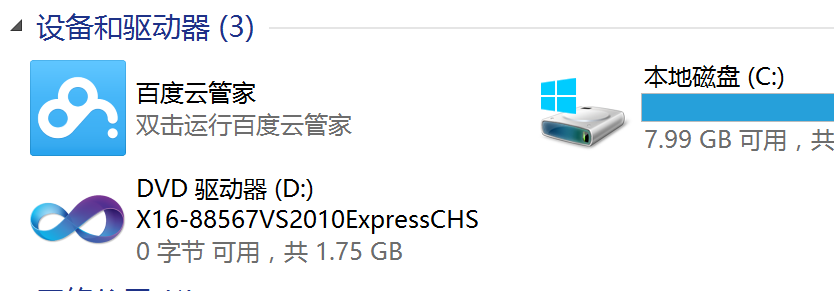
\includegraphics[width=0.5\hsize]{pic/p2.PNG}
	 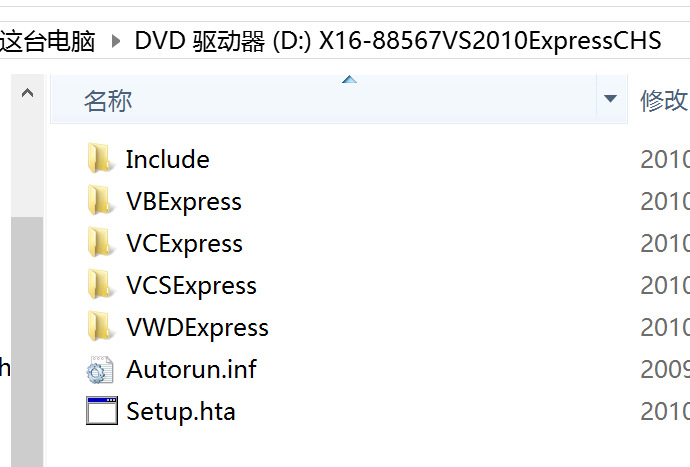
\includegraphics[width=0.5\hsize]{pic/pai.PNG}
	\end{center}
      }
      
      \only<3-8>{
	\begin{itemize}
	 \only<3>{\item 选择第三个 \textbf{visual C++ 学习版}}
	 \only<4-6>{\item \textbf{然后}}
	 \only<7>{\item 选择安装路径,可以放到D盘,但是还是会有小部分装在C盘}
	 \only<8>{\item 装好}
	\end{itemize}
	\begin{center}
	 \only<3>{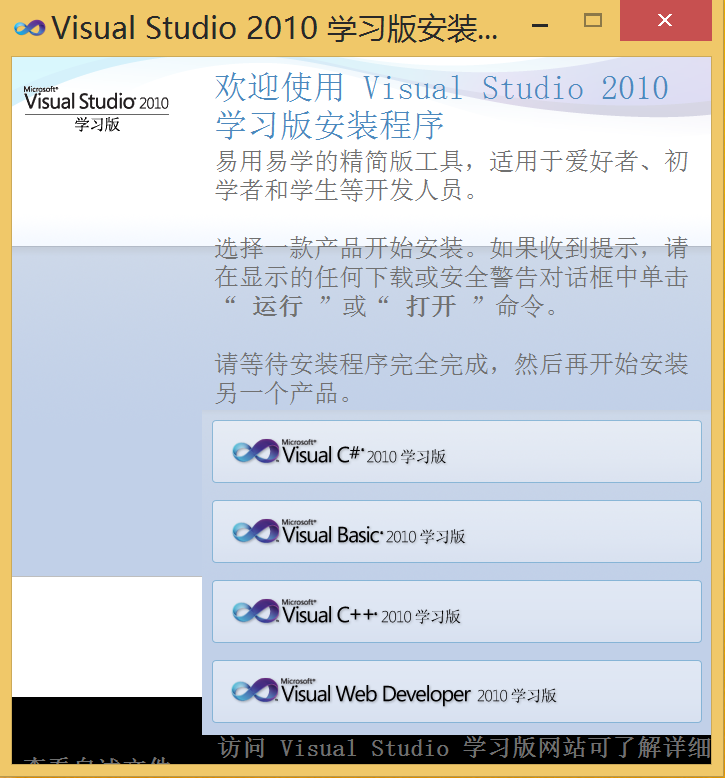
\includegraphics[width=0.7\hsize]{pic/p1.PNG}}
	 \only<4>{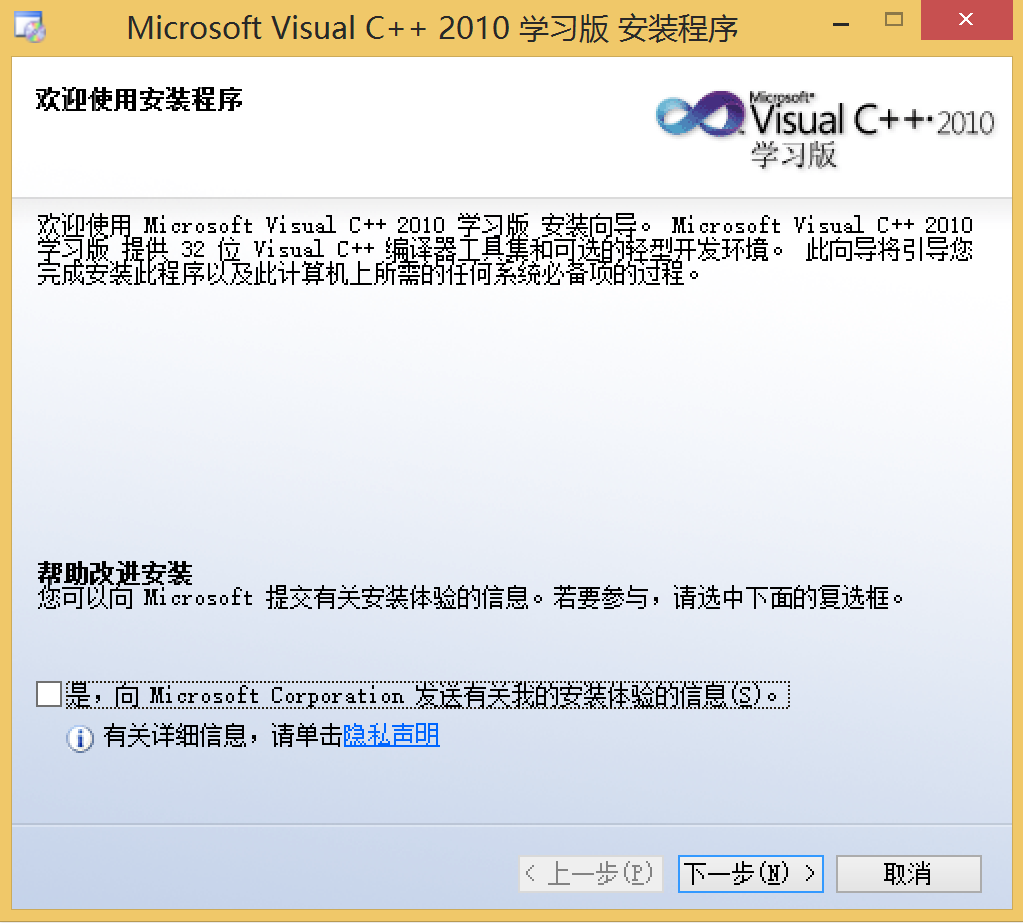
\includegraphics[width=0.8\hsize]{pic/P7.PNG}}
	 \only<5>{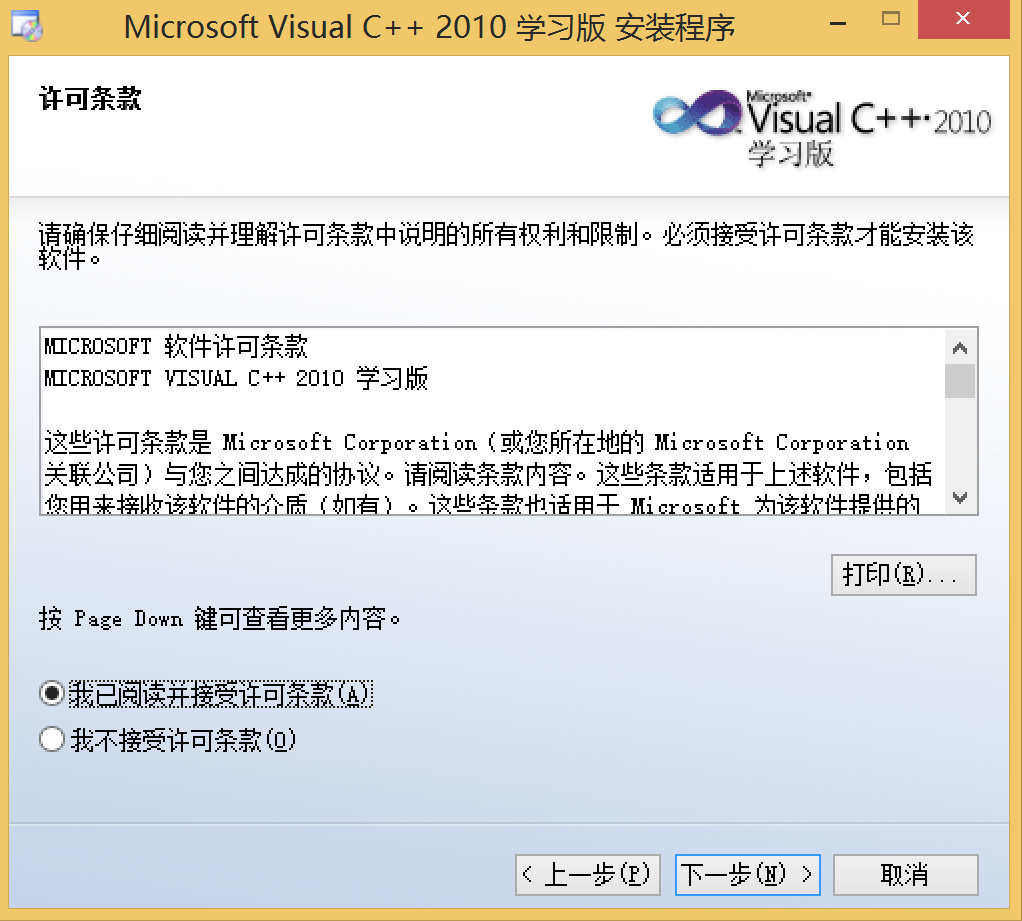
\includegraphics[width=0.8\hsize]{pic/P8.PNG}}
	 \only<6>{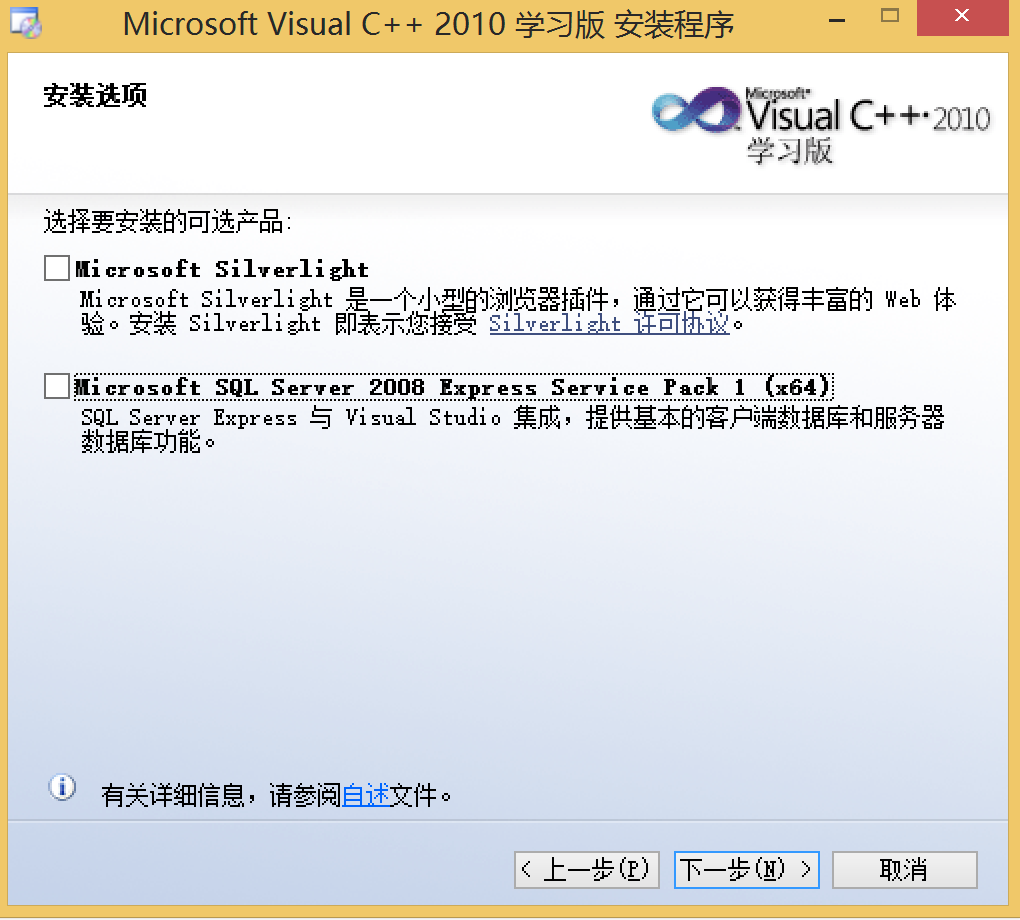
\includegraphics[width=0.8\hsize]{pic/P9.PNG}}
	 \only<7>{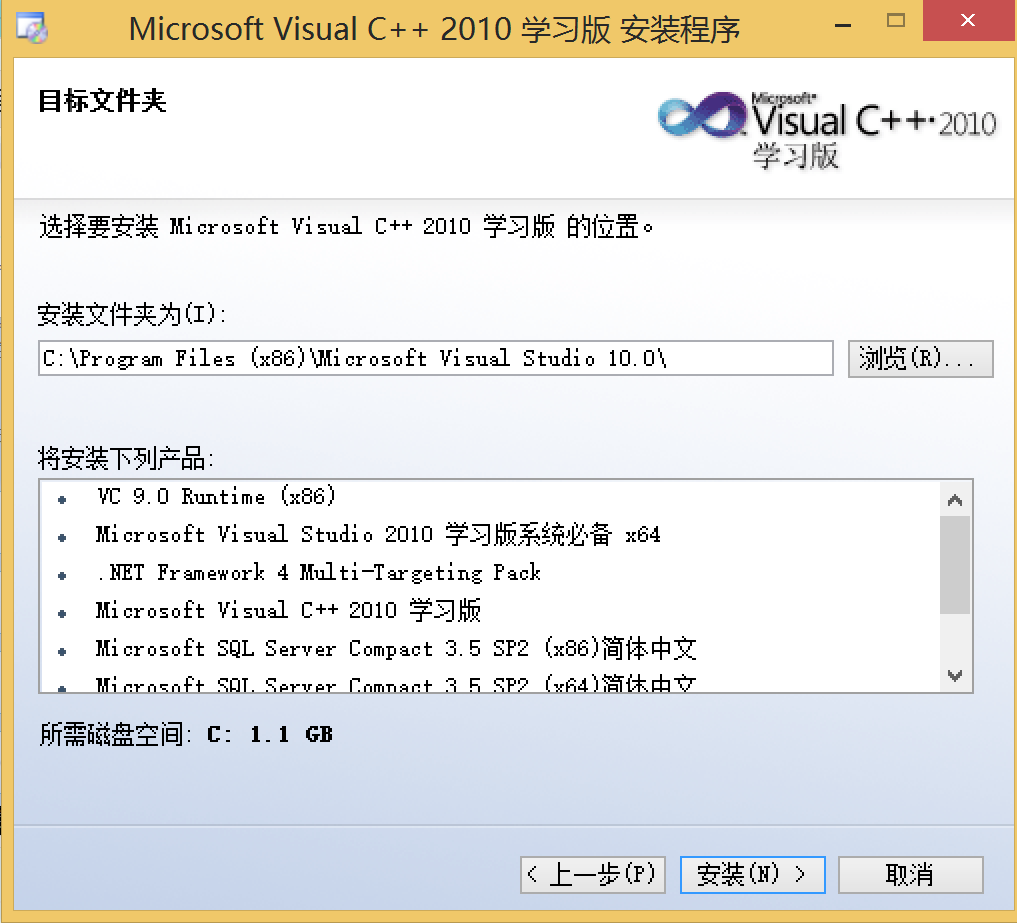
\includegraphics[width=0.75\hsize]{pic/p11.PNG}}
	 \only<8>{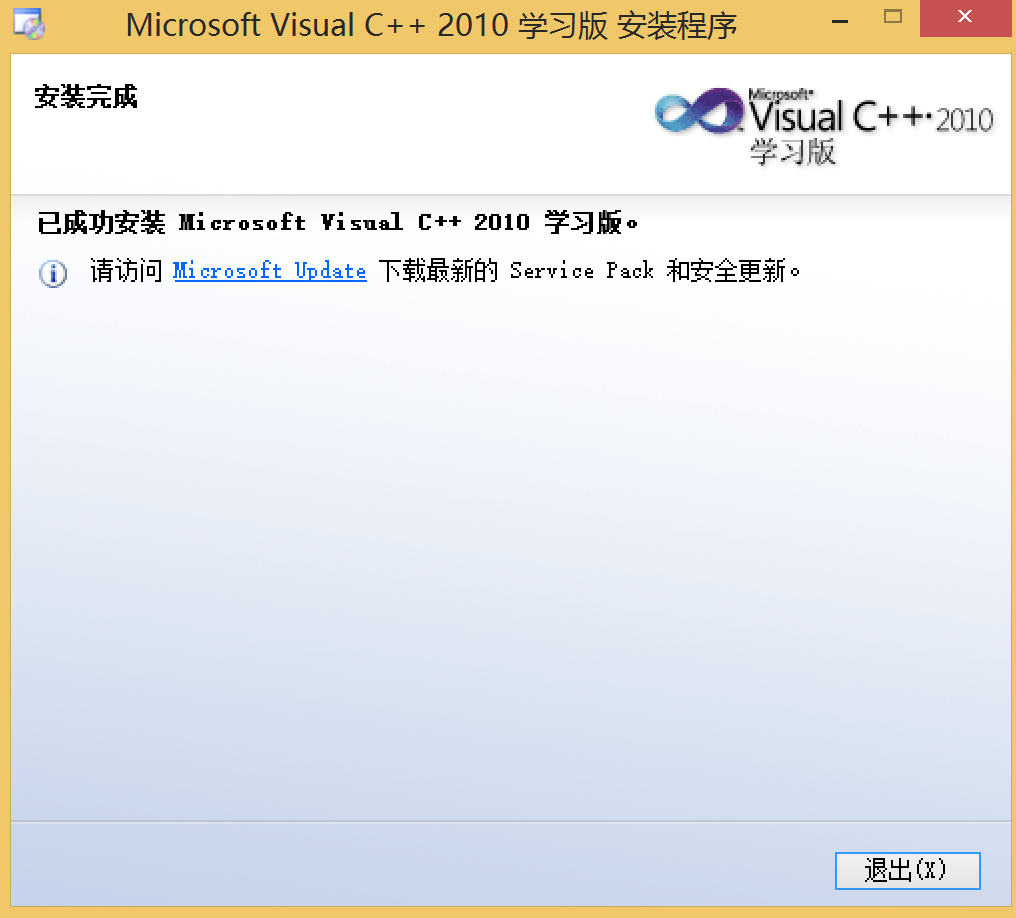
\includegraphics[width=0.75\hsize]{pic/p12.PNG}}
	\end{center}
      }
    \end{columns}	
}


\frame{
  \begin{columns}[c]
   \column{.15\hsize}
   \column{.7\hsize}
   \begin{block}{}
    \centering \Large 运行实例
   \end{block}

   \column{.15\hsize}
  \end{columns}

}

\frame{
  \frametitle{运行实例}
  \begin{columns}
   \column{0.25\hsize}
    \begin{block}{}
     \setbeamercovered{transparent}
     \begin{itemize}
      \item <1-4> {创建工程}
      \item <5-6> {创建c文件}
      \item <7> {运行代码}
      \item <8-> {调试/debug}
     \end{itemize}
    \end{block}
   
   \column{0.7\hsize}
   \only<1-7>{
    \begin{itemize}
     \only<1> {\item 新建项目}
     \only<2> {\item win32 控制台应用程序}
     \only<3> {\item 下一步}
     \only<4> {\item 选择 \textbf{空项目}}
     \only<5> {\item 源文件->添加->新建项}
     \only<6> {
	\item 选择 \textbf{C++} 文件, 并且文件名叫 \text{XXX.c}
	\begin{itemize}
	 \item c++的编译器可以兼容/支持c文件。所以可以直接写c语言文件
	\end{itemize}

     }
     \only<7> {
      \item 创建 test.c 如下,按 \red{\textbf{Ctrl+F5}} 运行即可
      \item 写完代码后在代码的某一行有红色下滑波浪线,说明代码\textbf{肯定}有问题,不用执行,直接查bug吧
     }
    \end{itemize}
   }
     \only<8> {
     \setbeamercovered{transparent}
      \begin{enumerate}
       \item <1-> {多在程序中间打印中间结果,尤其是代码没有输出/进入死循环时}
       \item <-.> {VS提示红色波浪线,说明代码不符合语法,肯定不能执行,看看大括号是不是匹配、变量使用之前是否已经定义、 ...}
      \end{enumerate}
     }
    \only<9>{
      \setbeamercovered{transparent}
      \begin{itemize}
       \item debug 断点调试\textbf{demo}
      \end{itemize}

    }
    \begin{center}
     \only<1> {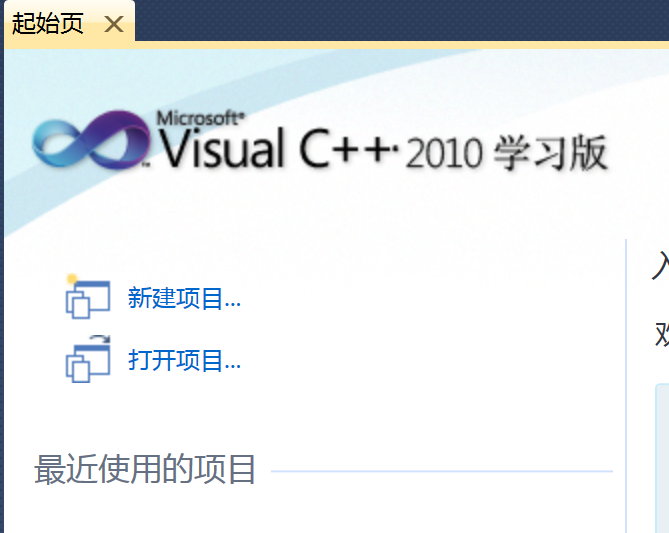
\includegraphics[width=0.65\hsize]{pic/p13.PNG}}
     \only<2> {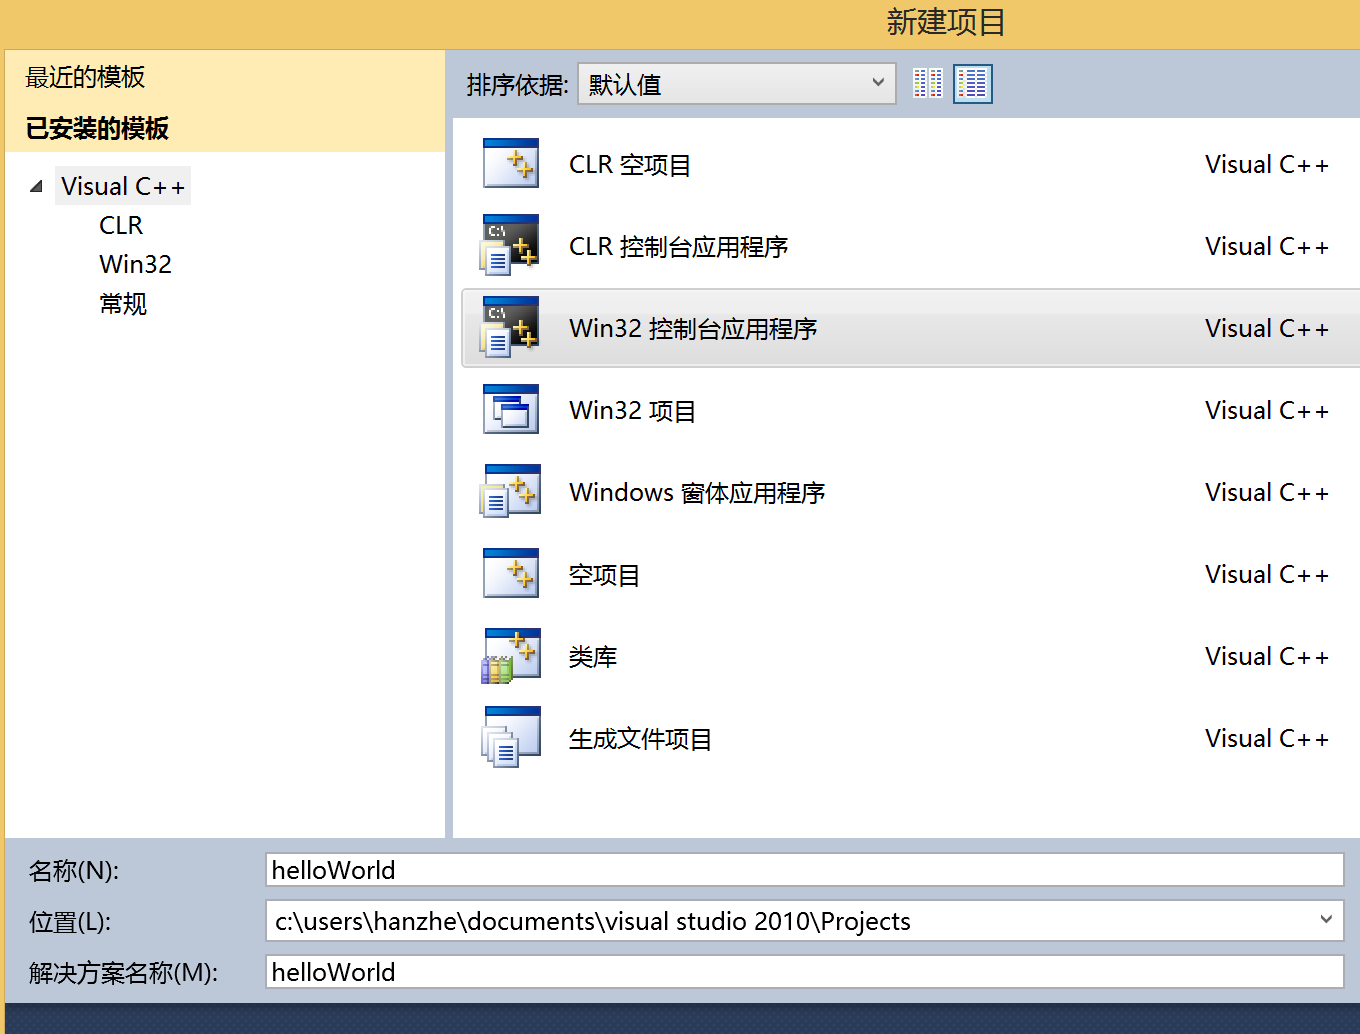
\includegraphics[width=0.85\hsize]{pic/p14.PNG}}
     \only<3> {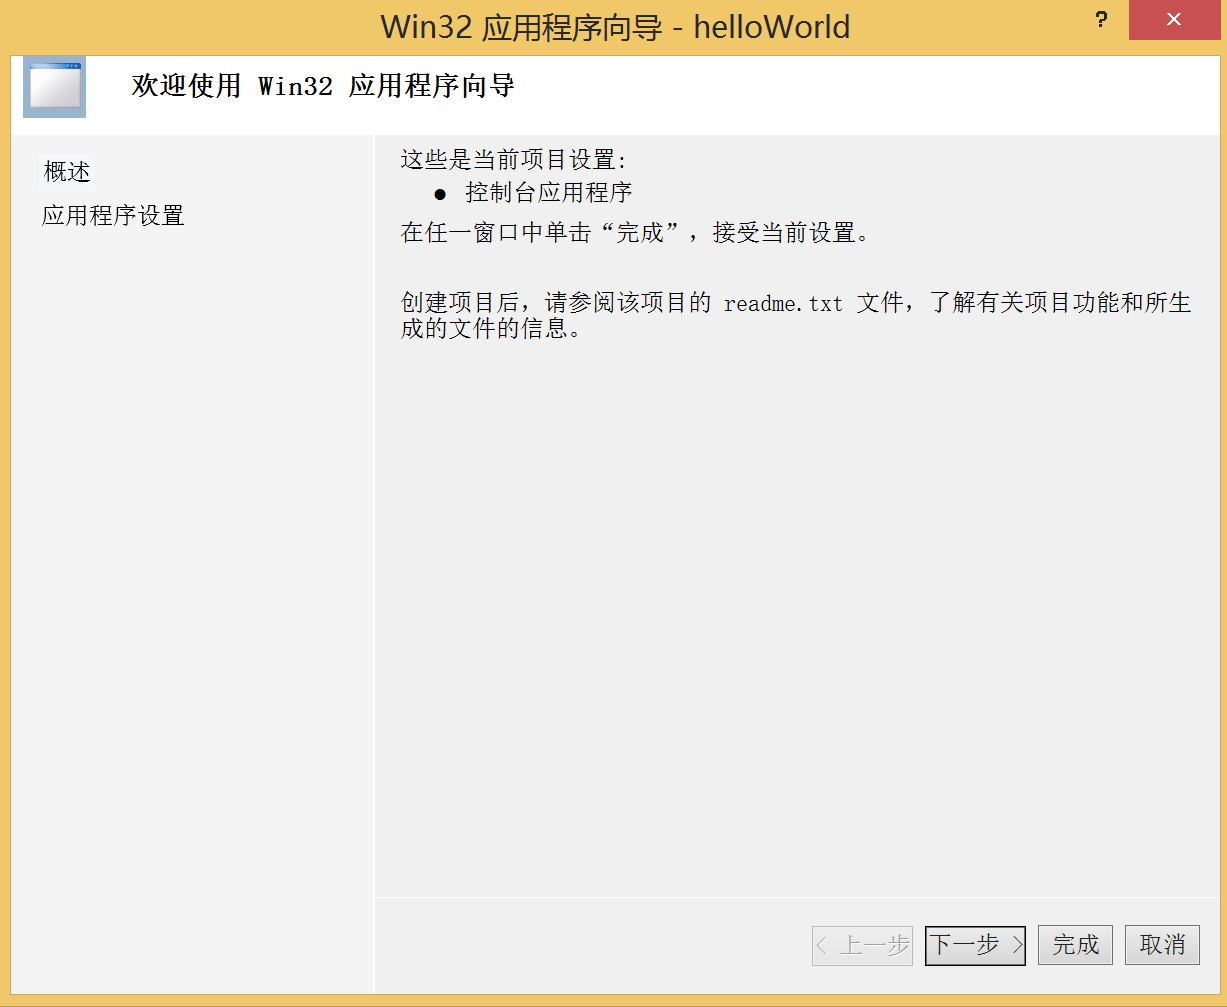
\includegraphics[width=0.85\hsize]{pic/p15.PNG}}
     \only<4> {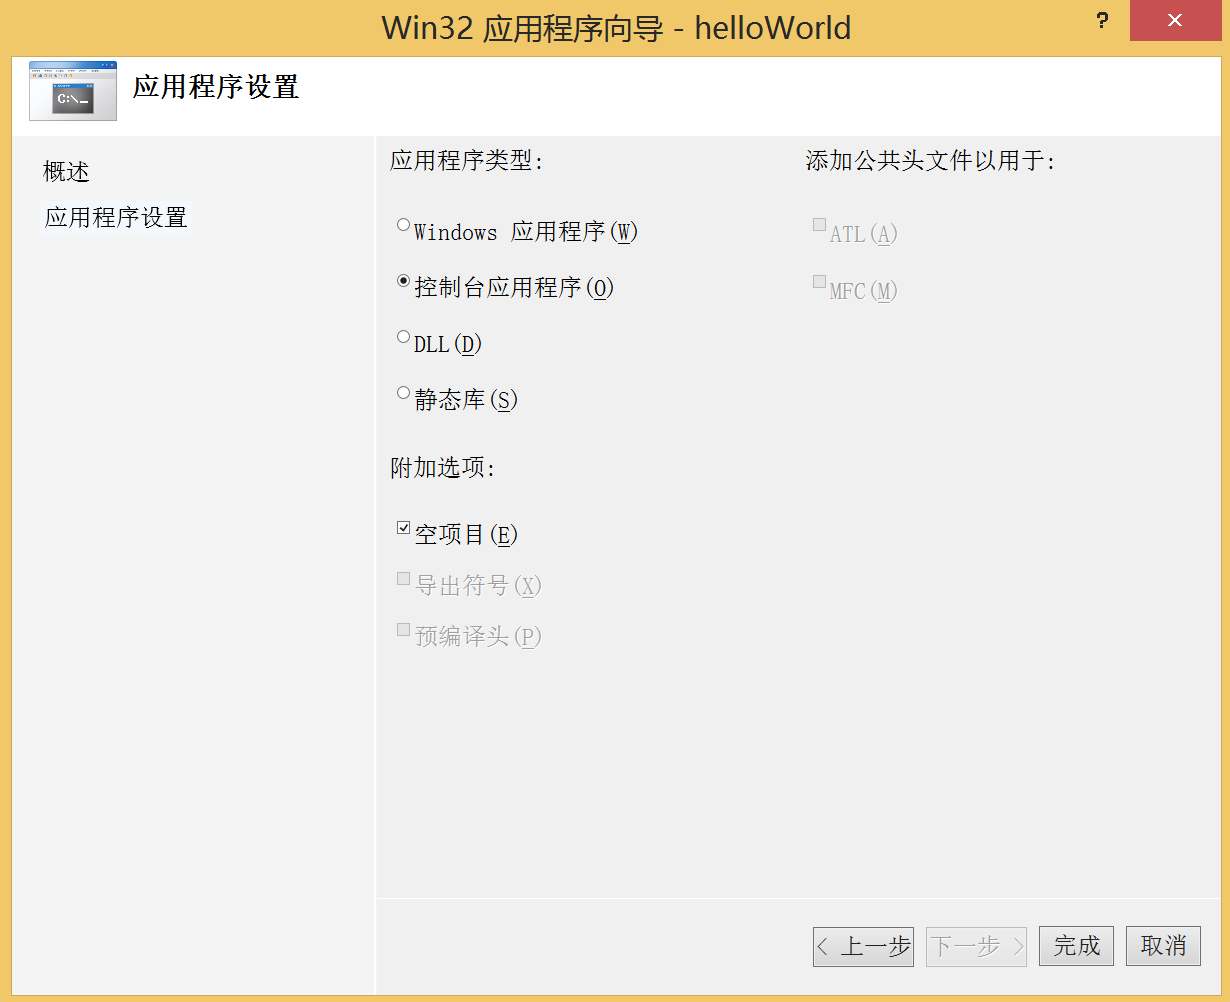
\includegraphics[width=0.85\hsize]{pic/p16.PNG}}
     \only<5> {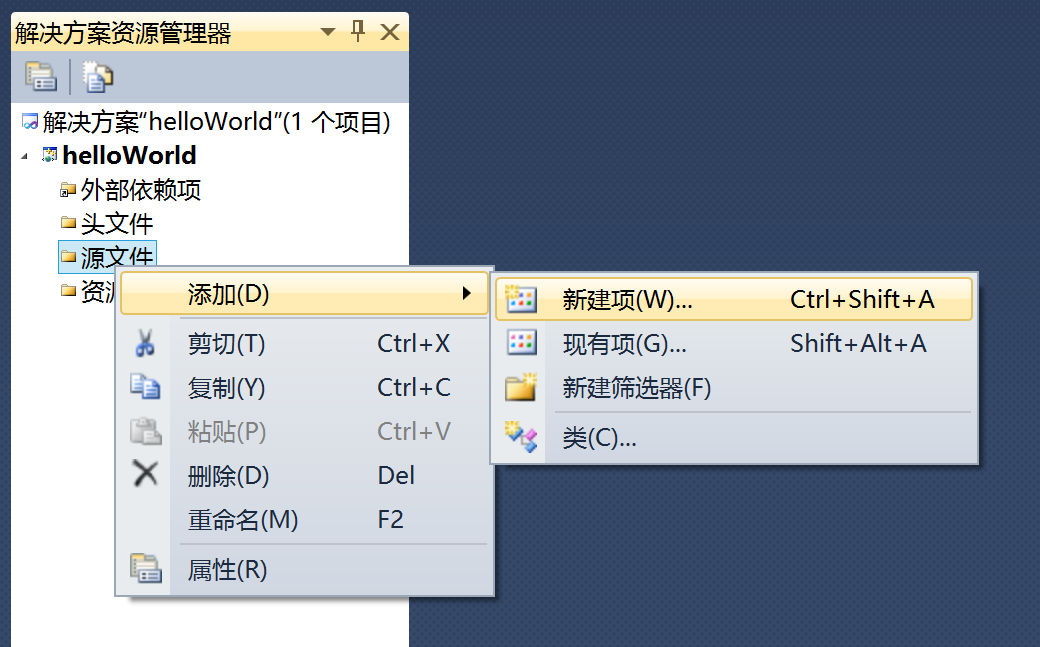
\includegraphics[width=0.85\hsize]{pic/p17.PNG}}
     \only<6> {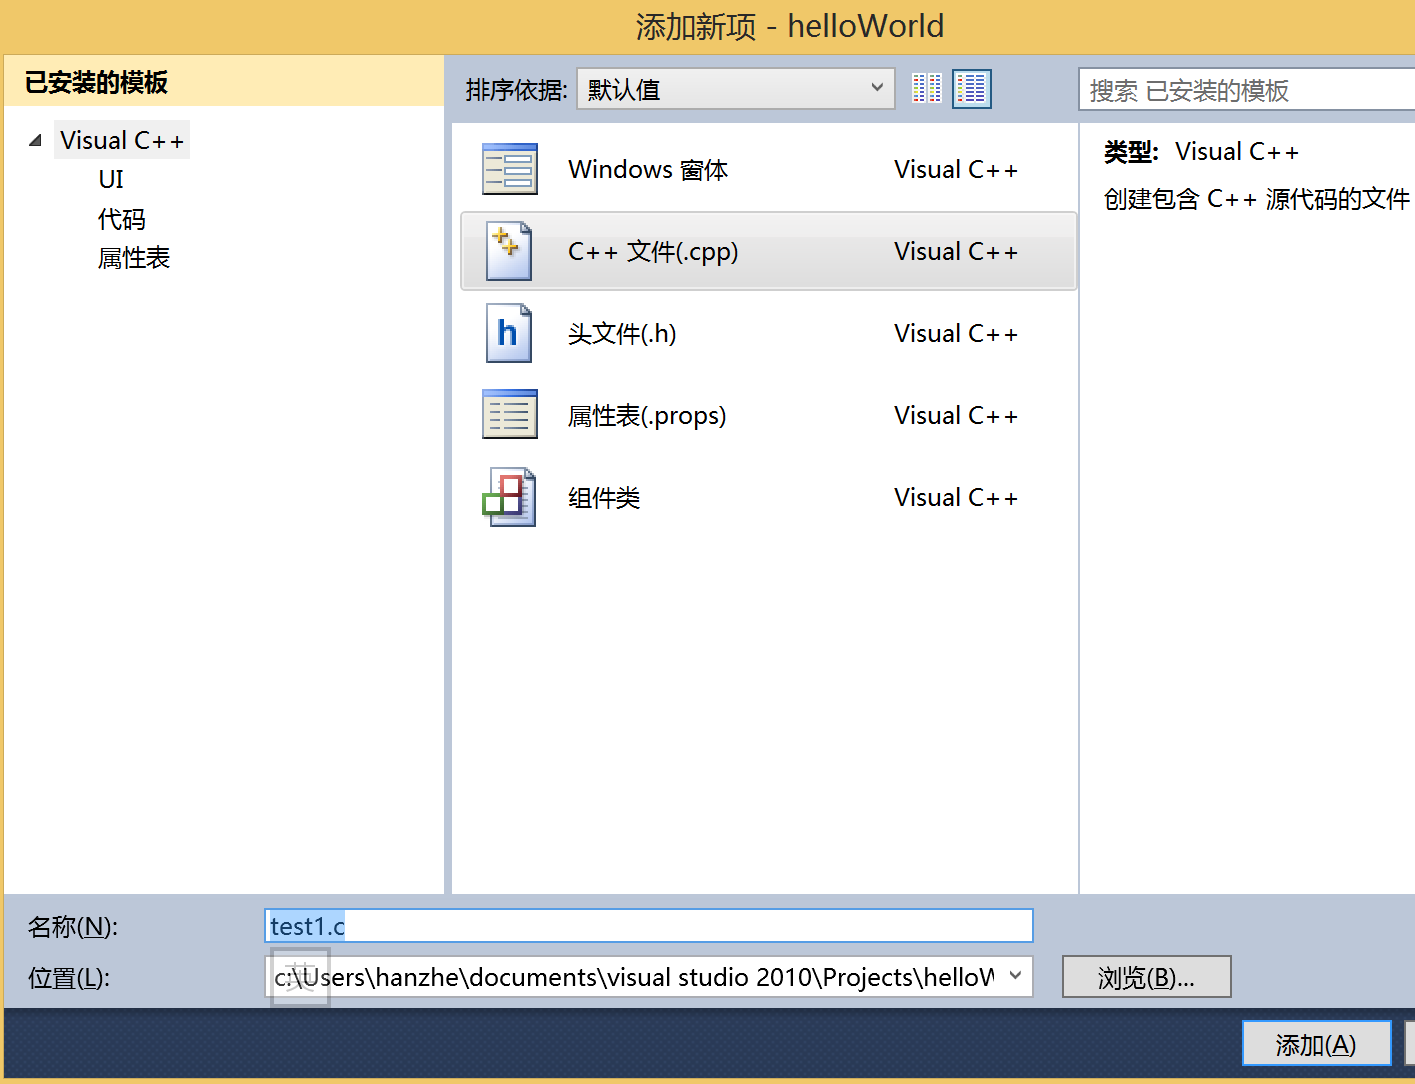
\includegraphics[width=0.85\hsize]{pic/p18.PNG}}
     \only<7> {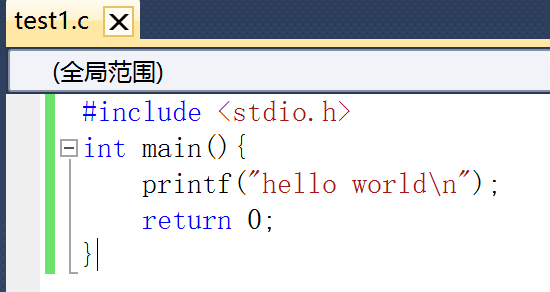
\includegraphics[width=0.85\hsize]{pic/p19.PNG}}
     \only<9> {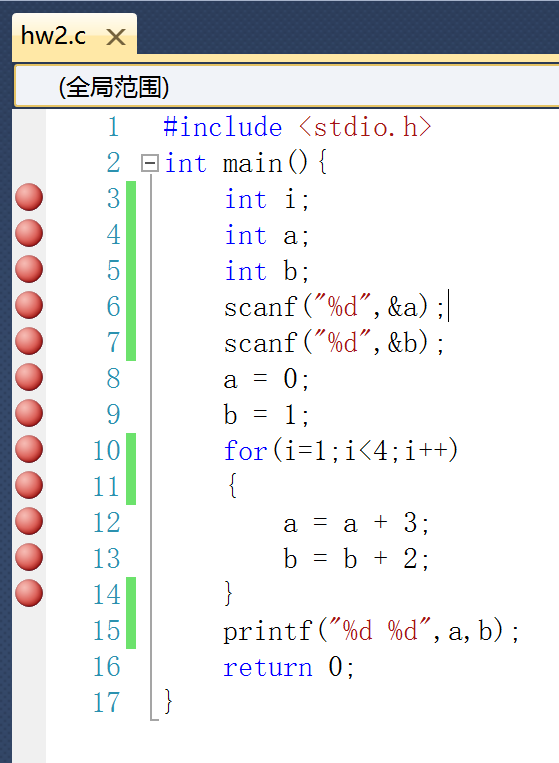
\includegraphics[width=0.75\hsize]{pic/p20.PNG}}
    \end{center}




  \end{columns}

}


\frame{
  \begin{columns}[c]
   \column{.15\hsize}
   \column{.7\hsize}
   \begin{block}{}
    \centering \Large 完全卸载vs2010express
   \end{block}

   \column{.15\hsize}
  \end{columns}

}

\frame{
  \frametitle{完全卸载vs2010express}
  \begin{itemize}
   \item 进入\textbf{控制面板},选择\textbf{删除程序}
   \item 按时间排序,把当天安装的微软的软件一个个删掉就行了
    \begin{itemize}
     \item 前提是当天没有安装其他微软软件
    \end{itemize}
  \end{itemize}
	\begin{center}
	 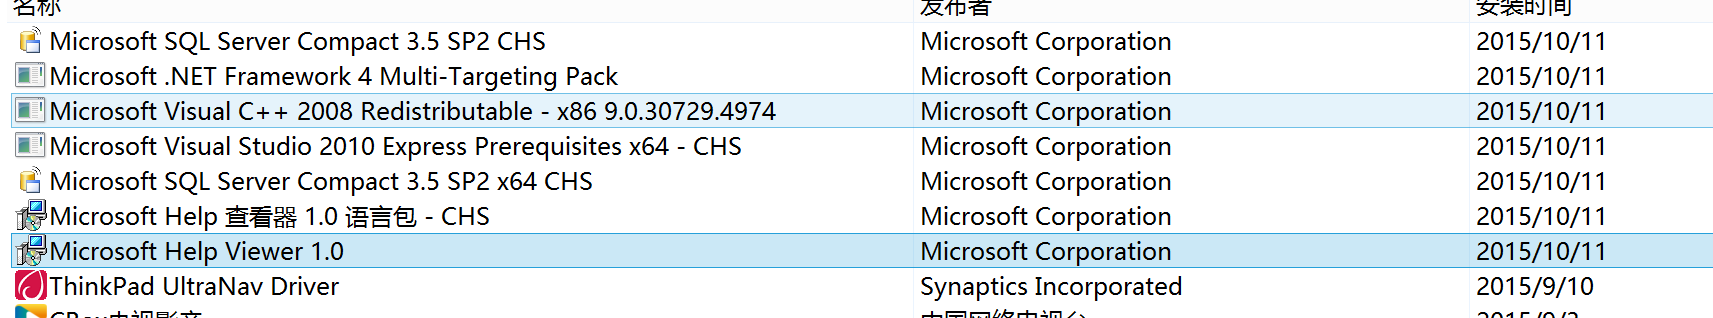
\includegraphics[width=0.9\hsize]{pic/p6.PNG}
	\end{center}
}

\frame{
  \begin{columns}[c]
   \column{.15\hsize}
   \column{.7\hsize}
   \begin{block}{}
    \centering \Large 谢谢大家!
   \end{block}

   \column{.15\hsize}
  \end{columns}

}


\frame{
  \frametitle{Appendix}
  \begin{columns}[c]
   \column{.15\hsize}
   \column{.7\hsize}
   \begin{block}{}
    \centering \Large Linux使用gcc在命令行下编译执行c程序
   \end{block}

   \column{.15\hsize}
  \end{columns}

}
\frame{
  \frametitle{Appendix: 安装gcc}
    \begin{block}{ubuntu14.04}
      \begin{enumerate}
       \item \textbf{Ctrl+Alt+T} 启动终端
       \item 输入`sudo apt-get install gcc`
      \end{enumerate}
    \end{block}
    
    \begin{block}{MacOS (我没有Mac...)}
      \begin{enumerate}
       \item 根据\href{http://stackoverflow.com/questions/9353444/how-to-use-install-gcc-on-mac-os-x-10-8-xcode-4-4}{google的答案}
       \item 启动终端,然后输入\textbf{xcode-select --install},安装 \textsl{command line tools}
      \end{enumerate}

    \end{block}
}

\frame{
  \frametitle{Appendix}
    \centering
    \begin{Large}
     命令行编译c程序
    \end{Large}
    
    \begin{columns}
     \column{0.1\hsize}
     
     \column{0.8\hsize}
     \begin{block}{}
      \begin{enumerate}
      \item \textbf{gcc} \red{源文件名称} \textbf{-o} \blue{编译后生成的可执行文件名称}
	\begin{itemize}
	 \item 确保终端当前所处的目录就是c文件所在目录
	\end{itemize}
     \end{enumerate}
     \end{block}
     \column{0.1\hsize}
    \end{columns}
}

\begin{frame}[fragile]
  \frametitle{Appendix: 命令行编译c程序}
  \begin{footnotesize}
  
  \begin{columns}
   \column{0.4\hsize}
\cCode
\begin{lstlisting}[frame=single]
#include <stdio.h>
int main(){
    printf("hello world!\n");
    return 0;
}
\end{lstlisting}

  
   \column{0.5\hsize}
   左边: hw.c \\
   
   左下: main.c \\ 
   右下: method.c (被main.c调用)
  \end{columns}

   

  \begin{columns}
   \column{0.4\hsize}
\cCode
\begin{lstlisting}[frame=single]
#include <stdio.h>
void multiPrint();
int main(){
    multiPrint();
}
\end{lstlisting}

  \column{0.5\hsize}
\cCode
\begin{lstlisting}[frame=single]
#include <stdio.h>
void multiPrint(){
    printf("hw1!\n");
    printf("hw2!\n");
    printf("hw3!\nhw4!\n");
    return;
}
\end{lstlisting}
  \end{columns}

  \end{footnotesize}
\end{frame}



\begin{frame}[fragile]
  \frametitle{Appendix: Ubuntu编译实例}
  
  \begin{columns}
   \column{0.3\hsize}
  \begin{footnotesize}
\cCode
\begin{lstlisting}[frame=single]
/* hw.c */
void multiPrint();
int main(){
    printf("hw!\n");
    return 0;
}
/* main.c */
int main(){
    multiPrint();
}
/* method.c */
void multiPrint(){
    printf("hw1!\n");
    printf("hw2!\n");
    printf("hw3!\n" +
      "hw4!\n");
    return;
}
 
\end{lstlisting}
  \end{footnotesize}

    \column{0.7\hsize}
    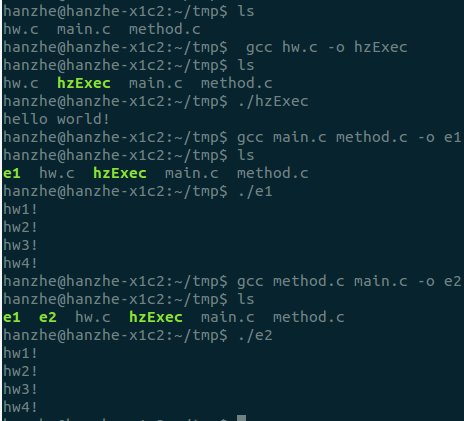
\includegraphics[width=1\linewidth]{ubuntu-gcc-demo.png}

   
  \end{columns}

\end{frame}


\end{document}

